% Content copied verbatim from KTVIC train_data.json, image_id 10954.
\begin{figure*}[t]
\centering
\begingroup
\setlength{\fboxsep}{4pt}
\definecolor{annotationkey}{RGB}{190,35,35}
\definecolor{annotationvalue}{RGB}{45,113,24}
\newcommand{\annotationpair}[2]{%
\noindent\textcolor{annotationkey}{\texttt{"caption":}} \textcolor{annotationvalue}{``#1''}\par
\noindent\textcolor{annotationkey}{\texttt{"segment\_caption":}} \textcolor{annotationvalue}{``#2''}\par}
\begin{minipage}[t]{0.25\textwidth}
\vspace{0pt}
\fbox{\begin{minipage}[c][5.1cm][c]{\dimexpr\linewidth-2\fboxsep-2\fboxrule\relax}
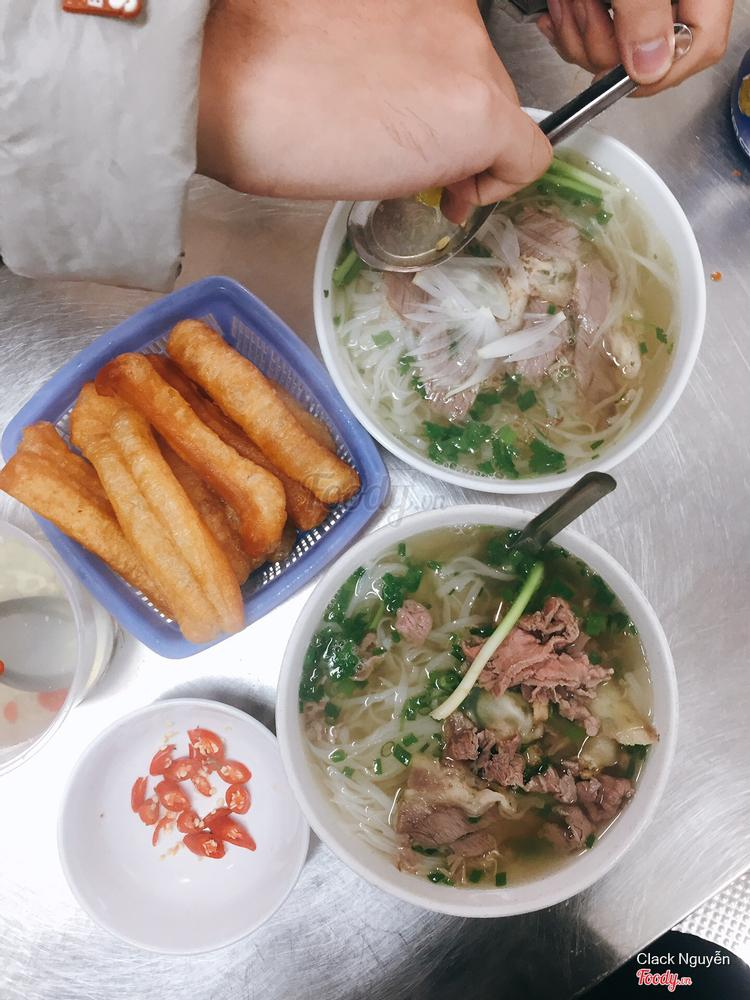
\includegraphics[width=\linewidth]{figures/ktvic_example_00000010954.jpg}
\end{minipage}}
\par\smallskip
\colorbox{black!8}{\parbox{\dimexpr\linewidth-2\fboxsep\relax}{\centering\small\texttt{image\_id: 10954}}}
\end{minipage}\hfill
\begin{minipage}[t]{0.72\textwidth}
\vspace{0pt}
\fbox{\begin{minipage}[c][5.1cm][s]{\dimexpr\linewidth-2\fboxsep-2\fboxrule\relax}
\fontsize{8.5}{10.5}\selectfont\raggedright
\annotationpair{có hai tô phở cùng một đĩa quẩy xuất hiện ở trên bàn}{có hai tô phở cùng một đĩa quẩy xuất\_hiện ở trên bàn}
\vfill
\annotationpair{có một người đang cầm trên tay một cái thìa}{có một người đang cầm trên tay một cái thìa}
\vfill
\annotationpair{có một cái muỗng xuất hiện ở trên tay của một người}{có một cái muỗng xuất\_hiện ở trên tay của một người}
\vfill
\annotationpair{có một đĩa quẩy được đặt ở bên cạnh hai bát phở}{có một đĩa quẩy được đặt ở bên cạnh hai bát phở}
\vfill
\annotationpair{có hai bát phở được bày ra ở trên bàn}{có hai bát phở được bày ra ở trên bàn}
\end{minipage}}
\par\smallskip
\colorbox{black!8}{\parbox{\dimexpr\linewidth-2\fboxsep\relax}{\centering\small Năm chú thích gốc và phiên bản tách từ}}
\end{minipage}
\endgroup
\caption{Ví dụ một mẫu ảnh và nhãn trong KTVIC: ảnh ID 10954 và đủ năm cặp chú thích.}
\label{fig:sample}
\end{figure*}
